\chapter{Diskussion}

\section{Oscillometrisk fikseret-ratio}
Den oscillometriske fikseret-ratio metode er brugt i hvid udstrækning til non-invasive målinger af det systoliske og diastoliske blodtryk. Det er derfor ikke unormalt at apparatet beskrevet i denne rapport under afsnit \ref{Fikseret-ratio}, anvender fikseret-ratio fastsat ud fra empirisk data. Flere studier har også vist at denne metode har en høj nøjagtighed.\fixme{Theory of the Oscillometric Maximum and the Systolic and Diastolic Detection Ratios} Problemet med denne rigide fortolkning at det systoliske og diastoliske blodtryk altid befinder sig samme procentsats fra middel arterie trykke opstår ved individernes forskellighed.

Jiankun et al\fixme{Error Mechanisms of the Oscillometric Fixed-Ratio BloodPressure Measurement Method} opstiller en matematisk model for den oscillometriske metode medregnet arterie eftergivenheden og undersøger ud fra dette hvilke faktorer, som påvirker den fikserede-ratio og hvor stor en afvigelse, fra den sande værdi dette giver. Resultaterne af denne gennemgang er teoretiske afvigelser på op til 58 mmHg ved svær arterie stivhed. Efter som at stive arterier ofte er til stede ved  arteriosklerose er apopleksi patienter (også beskrevet i afsnit \ref{chap:Baggrund}) særlig udsatte for fejlmålinger med fikseret-ratio metoden. Den korte forklaring på dette problem er ændringer af manchet oscillotionernes kurve brede. Kurven som dannes af peak ampletuderne af oscillotionerne (se figur \ref{fig:OscillometriskMetode}) ændre karakter ved ændring af arterie stivheden. Dette illustreres bedst ved at afbillede data med normaliseret manchettryk oscillotioner over manchettrykket på arterier forskellig eftergivenhed. 

\begin{minipage}[t]{0.5\textwidth}
På figur \ref{fig:ErrorMechanismOfFixedRatio} er fejl mekanismen ved fikseret-ratio bestemt systolisk tryk (SP) og diastolisk tryl (DP) illustreret. Peak ampletuderne er normaliseret, hvilket tydeliggør ændringerne i kurve bredden, når arterie eftergivenheden ændres. Ved normale arterievægge passer de empiriske ratio værdier godt, men efter som arteriet afviger fra det normale stiger fejl estimationen af SP og DP i takt med afvigelsen af eftergivenheden. Hvis er stiverer en normalt resulterer det i en overestimation af det systoliske tryk og en underestimation af det diastoliske tryk. Overestimationen finder sted fordi den konstante ratio for det systoliske tryk (SP/MAP) nu befinder sig på et tidligere tidspunkt i tid, hvor manchet trykket er højere og derfor overestimerers SP. På samme måde som systolisk tryk overestimeres, underestimeres det diastoliske tryk fordi den konstante ratio for det diastolisk tryk (SP/MAP) nu befinder sig på et senere tidspunkt i tid, hvor manchettrykket er laverer. Det samme scenarie gør sig gældende bare modsat, for en blodtryksmåling på arterier med en højere eftergivenhed end normalt. Ændringer i arterievæggens eftergivenhed påvirker ikke estimationen af MAP, som altid befinder sig med de største oscillotioner i manchetten.

Anvendelse af oscillometrisk fikseret-ratio metoden, til at måle blodtryk på patienter med apopleksi kan være problematisk på grund arterie stivheden, som giver anledning til fejl estimationer på op til 58 mmHg. Det bør derfor overvejes om andre metoder til at estimerer det sys- og diastoliske tryk skal anvendes i stedet, for at sikre en højere nøjagtighed af blodtryksmålingerne.

Overestimationen af det systoliske blodtryk optræder ikke som fejlkilde ved konditioneringen, da her blot ønskes en total okklution af arterierne. Overestimationen giver ikke anledning til et for lavt afklemningstryk, som tillader blod til den afklemte ekstremitet. Fejlkonditionering på grund af blodtryksmålingen opstår kun ved underestimering af SYS.
\end{minipage}
\begin{minipage}[t]{0.5\textwidth}
	\begin{figure}[H]
		\centering
		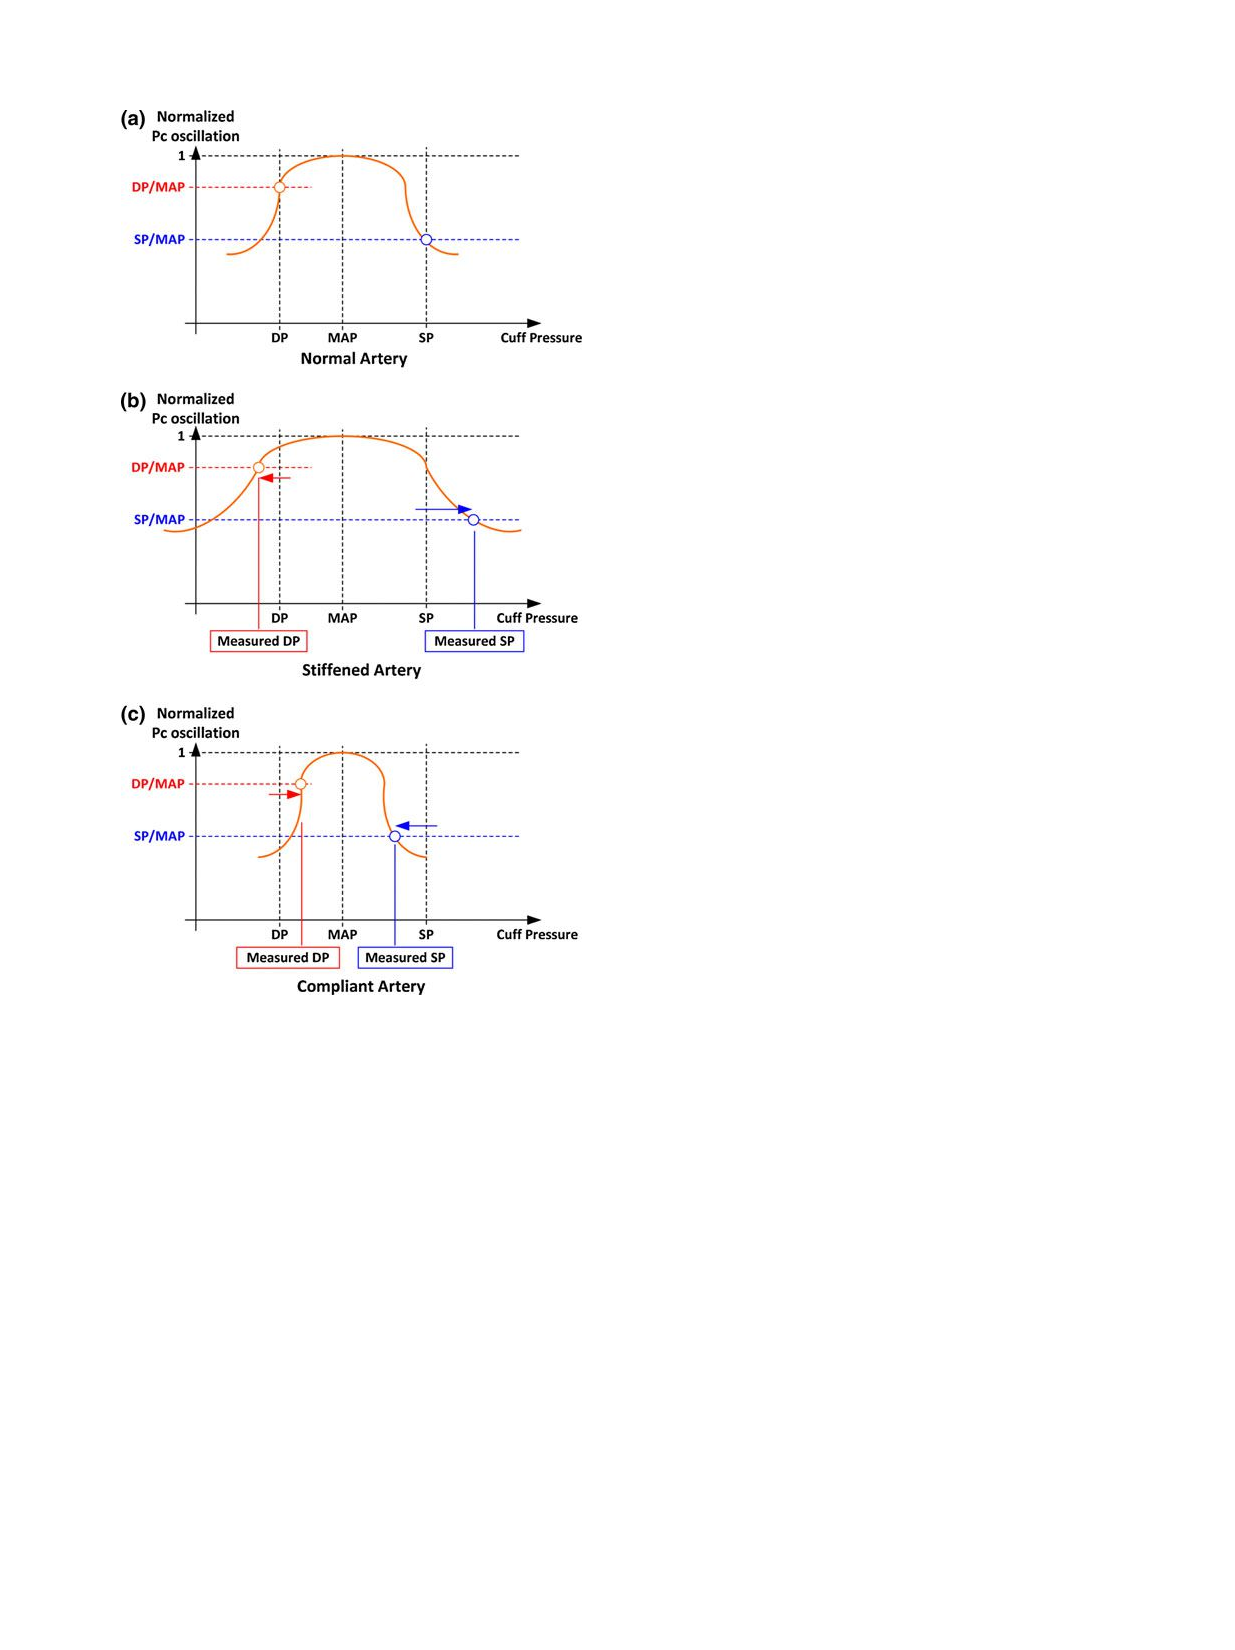
\includegraphics[width=1\textwidth]{billeder/ErrorFixed-Ratio.pdf}
		\caption{Fejl mekanismen i fixed-ratio metoden ved ændringer af arterie stivheden. Pc er manchet tryk. DP er det diastoliske tryk og SP er det systoliske tryk}\label{fig:ErrorMechanismOfFixedRatio}
	\end{figure}
	\fixme{billede Ref: Error Mechanisms of the Oscillometric Fixed-Ratio BloodPressure Measurement Method}
\end{minipage}




